% !TEX program = pdflatex
\documentclass[11pt,a4paper]{report}
\usepackage[T1]{fontenc}
\usepackage[utf8]{inputenc}
\usepackage[english]{babel}
\usepackage{lmodern}
\usepackage[scaled]{helvet}
\renewcommand{\familydefault}{\sfdefault}
\usepackage{microtype}
\usepackage[margin=2.5cm,headheight=14pt]{geometry}
\usepackage{xcolor}
\usepackage{graphicx}
\usepackage{booktabs,tabularx}
\usepackage{titlesec}
\usepackage{fancyhdr}
\usepackage{enumitem}
\usepackage[most]{tcolorbox}
\usepackage{pgfplots}
\pgfplotsset{compat=1.18}
\usepackage[hidelinks]{hyperref}

\definecolor{tocaInk}{HTML}{1E2127}
\definecolor{tocaHoney}{HTML}{D98E1F}
\definecolor{tocaGrey}{HTML}{6B7280}
\definecolor{tocaCream}{HTML}{FAF5EA}

% Chapters as numbered sections with a honey rule, no "Capítulo N" page.
\titleformat{\chapter}[hang]{\Huge\bfseries\color{tocaInk}}{\color{tocaHoney}\thechapter}{0.6em}{}[\vspace{2pt}{\color{tocaHoney}\titlerule[1.5pt]}]
\titlespacing*{\chapter}{0pt}{0pt}{1.4em}
\titleformat{\section}{\Large\bfseries\color{tocaInk}}{\thesection}{0.6em}{}
\setlist{itemsep=3pt}
\setlength{\parindent}{0pt}
\setlength{\parskip}{0.6em}

\pagestyle{fancy}
\fancyhf{}
\fancyhead[L]{\small\color{tocaGrey}{{TITLE}}}
\fancyhead[R]{\small\color{tocaGrey}{{INSTITUTION}}}
\fancyfoot[R]{\small\thepage}
\renewcommand{\headrulewidth}{0.4pt}
\fancypagestyle{plain}{\fancyhf{}\fancyfoot[R]{\small\thepage}\renewcommand{\headrulewidth}{0pt}}

\newtcolorbox{destaque}[1][]{colback=tocaCream,colframe=tocaHoney,boxrule=0pt,leftrule=3pt,arc=2pt,left=10pt,right=10pt,top=8pt,bottom=8pt,#1}

\begin{document}

% ---------------------------------------------------------------- capa
\begin{titlepage}
  \newgeometry{margin=0pt}
  \pagecolor{tocaInk}\color{white}
  \vspace*{6cm}
  \hspace*{2.5cm}\begin{minipage}{0.75\paperwidth}
    {\color{tocaHoney}\rule{3cm}{5pt}}\par\vspace{1cm}
    {\fontsize{34}{40}\selectfont\bfseries {{TITLE}}\par}\vspace{0.6cm}
    {\Large Report subtitle\par}\vspace{3cm}
    {\large {{AUTHOR}}\par}\vspace{0.2cm}
    {\color{tocaHoney}{{INSTITUTION}}\par}\vspace{0.2cm}
    {{DATE}}
  \end{minipage}
  \vfill
  \hspace*{2.5cm}{\small\color{tocaGrey}Confidential. Version 1.0}\par\vspace{2cm}
  \restoregeometry
\end{titlepage}
\nopagecolor\color{black}

% ---------------------------------------------------------------- sumário executivo
\chapter*{Executive summary}
\addcontentsline{toc}{chapter}{Executive summary}

\begin{destaque}
  \textbf{In one sentence:} what the report concludes and what it recommends.
\end{destaque}

\begin{itemize}
  \item \textbf{Finding 1.} Revenue grew 18\% over the year, led by the Northeast.
  \item \textbf{Finding 2.} Customer acquisition cost fell by half.
  \item \textbf{Recommendation.} Expand operations in the Northeast before the second half.
\end{itemize}

\tableofcontents

% ---------------------------------------------------------------- corpo
\chapter{Background}
Why the report was requested, what question it answers and what data it uses.

\chapter{Results}
\section{Revenue by region}
Figure~\ref{fig:receita} compares the regions and Table~\ref{tab:indicadores} summarizes the indicators.

\begin{figure}[h]
  \centering
  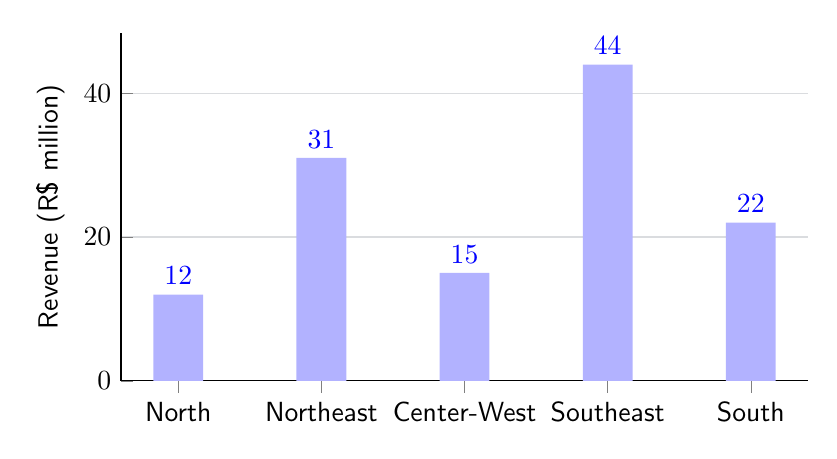
\begin{tikzpicture}
    \begin{axis}[
      ybar, bar width=18pt, width=0.85\linewidth, height=6cm,
      symbolic x coords={North,Northeast,Center-West,Southeast,South}, xtick=data,
      ylabel={Revenue (R\$ million)}, ymin=0, nodes near coords,
      axis lines*=left, ymajorgrids, grid style={tocaGrey!25},
      every axis plot/.append style={fill=tocaHoney, draw=none},
    ]
      \addplot coordinates {(North,12) (Northeast,31) (Center-West,15) (Southeast,44) (South,22)};
    \end{axis}
  \end{tikzpicture}
  \caption{Revenue by region in 2026.}\label{fig:receita}
\end{figure}

\section{Indicators}
\begin{table}[h]
  \centering
  \caption{Key indicators}\label{tab:indicadores}
  \begin{tabularx}{0.8\linewidth}{Xrrr}
    \toprule
    Indicator & 2025 & 2026 & Change \\
    \midrule
    Revenue (R\$ m) & 105 & 124 & +18\% \\
    Active customers (thousand) & 48 & 61 & +27\% \\
    Acquisition cost (R\$) & 210 & 104 & $-$50\% \\
    \bottomrule
  \end{tabularx}
\end{table}

\chapter{Recommendations}
\begin{enumerate}
  \item \textbf{Short term.} What to do in the next three months.
  \item \textbf{Medium term.} What to plan for the year.
  \item \textbf{Risks.} What could go wrong and how to track it.
\end{enumerate}

\appendix
\chapter{Methodology}
Data sources, definitions and limitations.

\end{document}
